
\chapter{User guide}\label{cha:UserGuide}

\section{Quick start guide}

\let\oldv\verbatim
\let\oldendv\endverbatim

\def\verbatim{\par\setbox0\vbox\bgroup\oldv}
\def\endverbatim{\oldendv\egroup\fboxsep0pt \noindent\colorbox[gray]{0.8}{\usebox0}\par}


The \FOLDING is a mechanism that provides instantaneous performance metrics, source code references and memory references\footnote{This last option is experimental at the moment of writing this document}.
This mechanism receives a trace-file (currently generated by \EXTRAE - see further details on generating a trace-file for the \FOLDING in Appendix~\ref{cha:GetATrace}) and generates plots and an additional trace-file depicting the fine evolution of the performance.
The \FOLDING uses information captured through instrumentation and sampling mechanisms and smartly combines them.
In this context, the samples are gathered from scattered computing regions into a synthetic region by preserving their relative time within their original region so that the sampled information determines how the performance evolves within the region.
Consequently, the folded samples represent the progression in shorter periods of time no matter the monitoring sampling frequency, and also, the longer the runs the more samples get mapped into the synthetic instance.
The framework has shown mean differences up to 5\% when comparing results obtained sampling frequencies that are two orders of magnitude more frequent.

\subsection{Decompressing the package}

The \FOLDING package is distributed in a .tar.bz2 file that can be uncompressed in the working directory by executing the following command:

\begin{verbatim}
# tar xvz folding-1.0rc8-x86_64.tar.bz2
\end{verbatim}

where \texttt{folding-1.0rc8-x86\_64.tar.bz2} refers to the \FOLDING package as distributed from the BSC web page\footnote{\url{http://www.bsc.es/computer-sciences/performance-tools/downloads}}.

\subsection{Contents of the package}\label{subsec:ContentsOfInstallation}

After decompressing the package, the working directory should be populated with the directories (and corresponding descriptions) as listed in Table~\ref{tab:contents_folding_package}.

\begin{table}
  \small
  \begin{center}
  \rowcolors{2}{tabbg2}{tabbg1}
  \caption{Contents of the folding package.}
  \label{tab:contents_folding_package}
    \begin{tabular}{l c l}
    \hlinethick
    Directory & & Contents \\
    \hline
    bin/ & & Binary packages \\
    etc/ & & \\
    \ \ extrae-configurations/ & & Minimal configuration files for \EXTRAE \\
    \ \ models/ & & Configuration files to calculate performance models \\
    \ \ \ \ basic/ & & \\
    \ \ \ \ ibm-power5/ & & \\
    \ \ \ \ ibm-power7/ & & \\
    \ \ \ \ ibm-power8/ & & \\
    \ \ \ \ intel-haswell/ & & \\
    \ \ \ \ intel-nehalem/ & & \\
    \ \ \ \ intel-sandybridge/ & & \\
    include/ & & Header files for the development of 3rd party tools \\
    lib/ & & Libraries for the folding \\
    share/ & & Miscellaneous files \\
    \ \ cfg/ & & Configuration files for Paraver \\
    \ \ doc/ & & Documentation\\
    \ \ \ \ html & & \\
    \ \ examples/ & & \\
    \ \ \ \ folding-writer/ & & Example on how to generate data for the folding \\
    \ \ \ \ user-functions/ & & Sample tracefile with manually instrumented regions \\
    \ \ \ \ clusters/ & & Sample tracefile with automatically detected regions \\
    \hlinethick
    \end{tabular}
  \end{center}
\end{table}


\subsection{Quick run}

This section provides examples of two types of execution of the \FOLDING tool.
These examples take benefit of the included sample trace-files from the package.
For further information on how to generate trace-files for the \FOLDING tool, check Appendix~\ref{cha:GetATrace}.

\subsubsection{Applied to manually instrumented regions}\label{subsubsec:ManualExample}

This first example uses a trace-file from the 444.namd SPEC benchmark that contains manually instrumented information that is located in 

\begin{verbatim}
${FOLDING_HOME}/etc/share/examples/user-functions
\end{verbatim}

This trace-file was generated by \EXTRAE and delimiting the main loop using the \EXTRAE API\footnote{Please refer to \url{http://www.bsc.es/computer-sciences/performance-tools/documentation} for the latest \EXTRAE User's Guide.}, more precisely the \texttt{Extrae\_user\_function} which emits events with label \texttt{User function} (or event type 60000019).
To apply the \FOLDING process to this trace-file, simply execute the following commands:

\begin{verbatim}
# cd ${FOLDING_HOME}/etc/share/examples/user-functions
# ${FOLDING_HOME}/bin/folding 444.namd.prv "User function"
\end{verbatim}

\subsubsection{Applied to automatically characterized regions}\label{subsubsec:ClusteredExample}

This example consists of a trace-file for the Nemo application when executed in MareNostrum3.
This trace-file contains information regarding automatically characterized regions.
This characterization has been done using the Clustering tool\footnote{Please refer to \url{http://www.bsc.es/computer-sciences/performance-tools/documentation} for the latest documentation with respect to the Clustering tool.}.
This tool enriches the trace-file by adding events labeled as \texttt{Cluster ID} (and event type 90000001) into the trace-file.
In this context, these events identify similar computation regions based on the event value.
To apply the \FOLDING process to this trace-file, simply execute the following commands:

\begin{verbatim}
# cd ${FOLDING_HOME}/etc/share/examples/user-functions
# ${FOLDING_HOME}/bin/folding \
  nemo.exe.128tasks.chop1.clustered.prv "Cluster ID"
\end{verbatim}

This trace-file also contains all the necessary performance counters in order to take benefit of several performance models based on performance counters.
Simply add the \texttt{-model intel-sandybridge} option to the \FOLDING script to generate the plots with information of the models instead of providing each performance counter individually.
The commands to execute should look like this:

\begin{verbatim}
# cd ${FOLDING_HOME}/etc/share/examples/user-functions
# ${FOLDING_HOME}/bin/folding -model intel-sandybridge \
  nemo.exe.128tasks.chop1.clustered.prv "Cluster ID"
\end{verbatim}

\subsection{Exploring the results}

The \FOLDING mechanism generates two types of output inside a directory named as the trace-file given (without the \texttt{.prv} suffix).
The first type of results include a set of gnuplot files where each of these represents the evolution of the performance counters within the region.
The tool also generates a \PARAVER trace-file with synthetic information derived from the \FOLDING mechanism.

\subsubsection{Using gnuplot}

With respect to the gnuplot files, the \FOLDING mechanism generates as many files as the combination of analyzed regions (clusters, OpenMP outlined routines, taskified OmpSs routines, or manually delimited regions) and the counters gathered during the application execution.
The user can easily list the generated gnuplot files calling \texttt{ls *.gnuplot} within the directory created.
The name of the gnuplot files contain the trace-file prefix, the identification of the region folded, and the performance counter shown.
For instance, the example described in Section~\ref{subsubsec:ManualExample} generates output files that can be explored by executing the command:

\begin{verbatim}
# gnuplot -persist \
  444.namd.codeblocks.fused.any.any.any.main.Group_0.PAPI_TOT_INS.\
  gnuplot
\end{verbatim}

When executing the aforementioned command, the \texttt{gnuplot} command should open a window that resembles that in Figure~\ref{fig:444_namd_instructions}\footnote{Warning! If the user has problems to open the gnuplot, they should check whether the gnuplot installation is compatible and supports the default terminal. Otherwise, simply select the appropriate terminal (or leave it blank) in the first four lines in the gnuplot script}.
The Figure shows that the application faces six phases that execute at 4,500~MIPS approximately.
Most of the code occurs in three code locations (being line 76 the most observed line), and we also observe that phases related to high MIPS are related with the activity in the middle of the code-line plot.

\begin{figure}
  \centering
  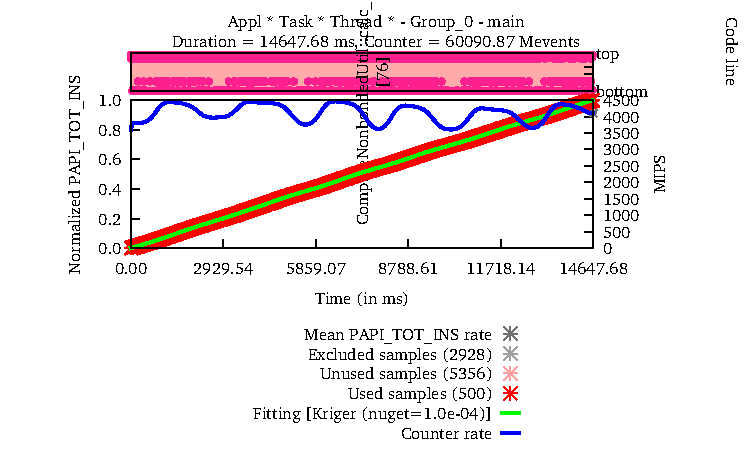
\includegraphics[width=0.65\textwidth]{figures/user-guide/444_namd_tot_ins.pdf}
  \caption{Evolution of graduated instructions for 444.namd.}
  \label{fig:444_namd_instructions}
\end{figure}


This file refers to the user routine \texttt{main} (which was manually instrumented) of the trace-file 444.namd.prv and provides information of the total graduated instructions (\texttt{PAPI\_TOT\_INS}). 
The user will notice that there are additional files for the different performance counters and they can explore them individually.
The \FOLDING also generates an additional plot that combines the metrics of all the counters into a single plot.
This plot mainly provides information with respect to the MIPS rate (referenced on the right Y-axis), and ratio of the remaining performance counters per instruction (referenced on the left Y-axis).
For the particular case of the example from Section~\ref{subsubsec:ManualExample}, this plot can be explored calling:

\begin{verbatim}
# gnuplot -persist \
  444.namd.codeblocks.fused.any.any.any.main.\
  Group_0.ratio_per_instruction.gnuplot
\end{verbatim}

This command should generate an output combining all the performance counter slopes as shown in Figure~\ref{fig:444_namd_ratio_per_instruction}.

\begin{figure}
  \centering
  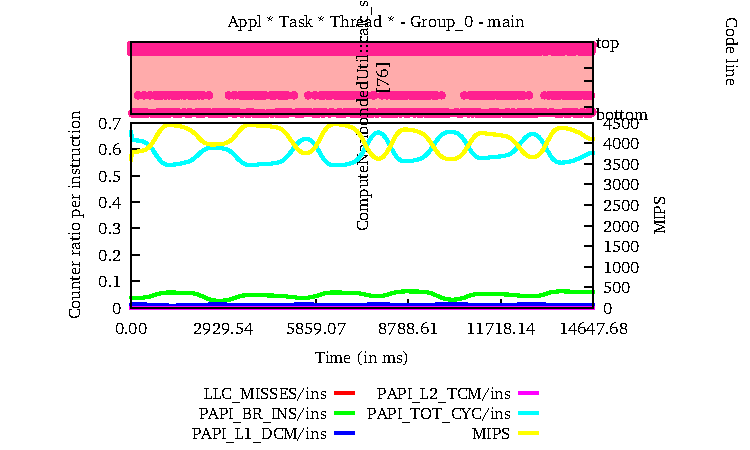
\includegraphics[width=0.65\textwidth]{figures/user-guide/444_namd_ratio_per_instruction.pdf}
  \caption{Evolution of multiple counters for 444.namd.}
  \label{fig:444_namd_ratio_per_instruction}
\end{figure}


The aforementioned instructions also apply to the automatically delimited example described in Section~\ref{subsubsec:ClusteredExample}.
In this case, the region names are numbered as \texttt{Cluster\_1} to \texttt{Cluster\_11}, but they also contain the trace-file prefix and the performance counters to explore them individually.
If the user requested the performance models, then additional gnuplot files are created to provide information regarding these models.
For the particular case of the Intel SandyBridge model, it generates three models that always generate the MIPS rate and add different metrics:

\begin{itemize}
	\item \textit{instruction-mix}\\
	Gives insight of the type of instructions executed along the region.
	\item \textit{architecture-impact}\\
	Provides information regarding to the cache misses at different levels and the branch mispredicts along the region.
	\item \textit{stall-distribution}\\
	This plot shows information regarding on which components of the processor are stalling the processor pipeline.
\end{itemize}

For instance, to open the instruction mix for the region labeled as Cluster 1 of the Nemo application executed in Section~\ref{subsubsec:ClusteredExample}, the user needs to open the plot invoking the commands below and should obtain a plot similar to Figure~\ref{fig:Nemo_cluster1_instructionmix}.
The reader may see that the application shows two distinctive phases (green and blue) and within each of them there are two repetitions of the same performance.

\begin{verbatim}
# gnuplot -persist \
  nemo.exe.128tasks.chop1.clustered.codeblocks.fused.any.any.any.\
  Cluster_1.Group_0.instructionmix.gnuplot
\end{verbatim}

\begin{figure}
  \centering
  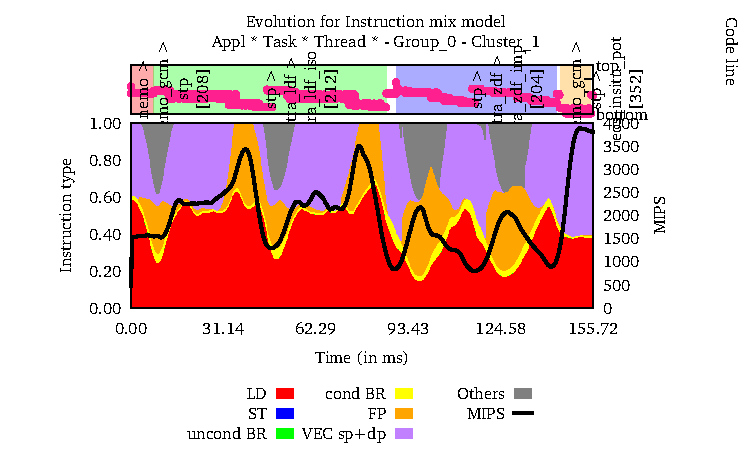
\includegraphics[width=0.65\textwidth]{figures/user-guide/nemo_cluster1_instructionmix.pdf}
  \caption{Instruction mix decomposition for Cluster 1 of Nemo.}
  \label{fig:Nemo_cluster1_instructionmix}
\end{figure}


The tool also provides a GUI-based tool to explore the plots. 
the user may invoke a visualizer named \texttt{wxfolding-viewer}, by invoking it from the newly created directory such as:

\begin{verbatim}
# ${FOLDING_HOME}/bin/wxfolding-viewer *.wxfolding
\end{verbatim}

\subsubsection{Using Paraver}

The \FOLDING process generates a trace-file with a suffix \texttt{.folded.prv} that lets \PARAVER to display some parts of the folded results.
The \FOLDING package includes several configuration files in the \texttt{\$\{FOLDING\_HOME\}/share/cfg} directory for \PARAVER to help analysing the results.
From the configuration files contained in that directory, we outline the following:

\begin{itemize}
	\item \textit{views}/
	\begin{itemize}
		\item \texttt{win\_folded\_type.cfg}\\
		Generates a time-line that shows in which instances the \FOLDING results have been integrated. This helps correlating the original trace-file and its contents with the folded trace-file. Notice that only one instance per type (where type refers to function, cluster, \textit{etc...}) is folded.
		\item \texttt{win\_folded\_mips.cfg}\\
		Generates a time-line showing a signal of the MIPS rate within the folded instances. See in Figure~\ref{fig:444_namd_instructions_paraver} a time-line depicting the MIPS rate achieved in the example trace-file for 444.namd.
		\item \texttt{win\_folded\_processed\_call-stack\_caller.cfg}\\
		Generates a time-line showing the most time-dominant routines as they have been executed within the folded instances. Figure~\ref{fig:Nemo_cluster1_callers_paraver} shows a time-line depicting the called routines for the Nemo example.
		\item \texttt{win\_folded\_processed\_call-stack\_callerline.cfg}\\
		Generates a time-line showing the most time-dominant source code references (as pair of line and file) as they have been executed within the folded instances.
	\end{itemize}
	\item \textit{histograms}/
	\begin{itemize}
		\item \texttt{3dh\_folded\_mips\_per\_caller.cfg}\\
		Generates a histogram that shows the achieved MIPS rate depending on the caller (columns) for a particular region folded.
		\item \texttt{3dh\_folded\_mips\_per\_callerline.cfg}\\
		Generates a histogram that shows the achieved MIPS rate depending on the source code references (pair of line and file in columns) for a particular region folded.
	\end{itemize}
\end{itemize}

\begin{figure}
  \centering
  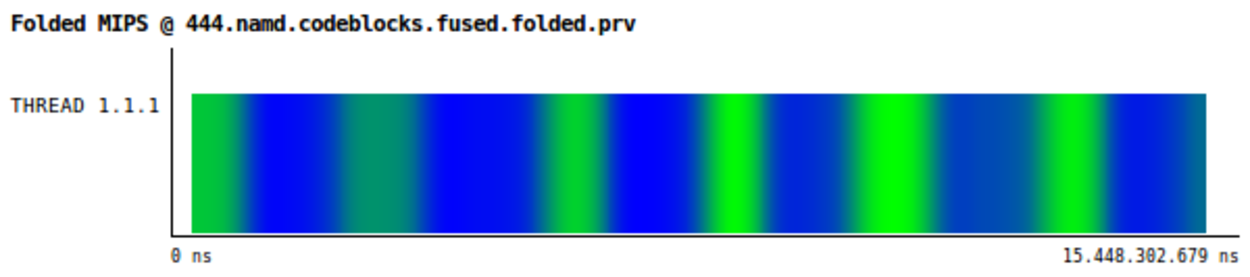
\includegraphics[width=0.75\textwidth]{figures/user-guide/444_namd_tot_ins_paraver.pdf}
  \caption{Evolution of graduated instructions for 444.namd in Paraver.}
  \label{fig:444_namd_instructions_paraver}
\end{figure}


\begin{figure}
  \centering
  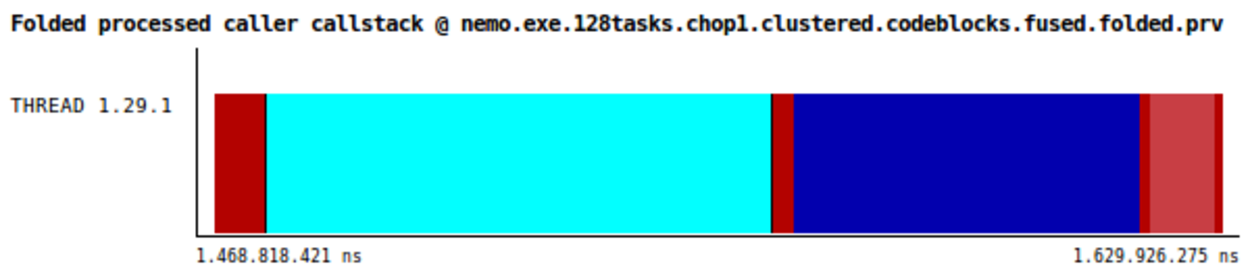
\includegraphics[width=0.75\textwidth]{figures/user-guide/nemo_cluster1_caller_paraver.pdf}
  \caption{Paraver time-line showing the callers for Cluster 1 of Nemo.}
  \label{fig:Nemo_cluster1_callers_paraver}
\end{figure}


\section{Configuration, build and installation}

This section describes how to build and install the \FOLDING package.
The \FOLDING package (and its dependencies) requires the Boost library (only the headers suffice), a C compiler, a Fortran compiler and a C++ compiler that supports the C++ 2011 specification (such as g++ version 4.8).
This package optionally uses the \texttt{strucchange} package from the R statistical application (and may execute in parallel if the \texttt{doParallel} is available) to use the piece-wise linear regression interpolation mechanism.
Additionally, the \FOLDING package requires the libtools package to be installed.
This package helps on the parsing of Paraver trace-files and can be downloaded from the BSC download web page.

\subsection{Libtools package}~\label{subsec:LibtoolsInstallation}

This package can be downloaded from the BSC web page and requires the boost header files\footnote{The libtools package has been successfully tested against version from 1.48 to 1.54.}.
If the boost header files are located in the system's default, simply run the following command:

\begin{verbatim}
# ./configure --prefix=/home/harald/aplic/libtools/1.0 \
  && make && make install
\end{verbatim}

where \texttt{--prefix} indicates the destination folder for this package.

If the boost header files are located elsewhere in the system, run the following command:

\begin{verbatim}
# ./configure --prefix=/home/harald/aplic/libtools/1.0 \
  --with-boost=/path/to/boost \
  && make && make install
\end{verbatim}

\subsection{Folding package}

The most basic configuration for the \FOLDING package honors the following commands:

\begin{verbatim}
# ./configure --with-libtools=$HOME/aplic/libtools/1.0 \
  --prefix=$HOME/aplic/folding/1.0rc8 && \
  make && make install
\end{verbatim}

where \texttt{--with-libtools} refers to the location of the libtools package installed in Section~\ref{subsec:LibtoolsInstallation} and \texttt{--prefix} indicates where to install the \FOLDING tool.
If the compilation and installation succeed, the contents of the target installation should look like as the contents defined in Section~\ref{subsec:ContentsOfInstallation}.

The \FOLDING tool supports several compilation flags that modify the behavior or enable additional functionalities of the tool.
The following list groups the flags according to the behavior they enable.

\begin{itemize}

	\item \texttt{--with-clustering-suite=<DIR>}\\
    The \FOLDING tool relies on the similarity between the folded instances in order to generate its results. By default, the \FOLDING tool includes two mechanisms to reduce the noise that appear from using instances with significant different behavior. However, this flag allows using the BSC Clustering suite as a third alternative in order to reduce the noise.

	\item \texttt{--with-R=<DIR1>, --with-cube=<DIR2>, --with-clang=<DIR3>}\\
	Enables the usage of piece-wise linear regressions on top of the strucchange package\footnote{\url{http://cran.r-project.org/web/packages/strucchange/index.html}} from the R statistical application\footnote{\url{http://www.r-project.org}}. This functionality requires the clang compiler\footnote{\url{http://clang.llvm.org}} and can generate input files for the Cube3 performance analysis package\footnote{\url{http://www.scalasca.org/software/cube-3.x/download.html}}.

	\item \texttt{--with-boost=<DIR>}\\
	This flag lets the \FOLDING to use a given Boost installation package.

	\item \texttt{--enable-gui}\\
	The results of the \FOLDING tool is a set of gnuplot files that have to explored manually. If this flag is given at the configure step, the \FOLDING package would include a GUI written in Python that helps exploring all the results from the tool.

	\item \texttt{--enable-callstack-analysis}\\
	This flag enables the call-stack analysis of the segments captured during the measurement step. Enabling this option results in gnuplot files that depict the performance progression collocated with the source code progression.

	\item \texttt{--enable-reference-analysis}\\
	This flag enables the memory references analysis of the references captured during the measurement step (currently, through the \texttt{perf} system tool). Enabling this option results in gnuplot files that depict the performance progression collocated with the memory address space and the sampled references.

\end{itemize}

